% !TeX spellcheck = en_GB
\chapter{Concept} % Lösungsentwurf 
\epigraph{Perfection (in design) is achieved not when there is nothing more to add,\\but rather when there is nothing more to take away.}{Antoine de Saint-Exupery}

% (Lösungsvarianten und deren Beurteilung, Variantenentscheid, Konzept, Entwurf)
% See arch. decisions

\section{Architecture}
% - Architekturdiagramme inkl. Layering (C4, UML)
% - mit Entscheidungen und begründung
% - wie Qualitätsattribute sichergestellt wurden
% - Beschreibung des Entwurfs (welche Experimente/Tests wurden durchgeführt? welche Lösungsoptionen wurden verworfen?)
% - Entwurf Benutzerschnittstelle

In this chapter, we present the architecture and fundamental architectural decisions of the XMPP grid broker application.
All architectural decisions we took are fully documented in Appendix~\fullref{sec:architectural-decisions}.

We illustrate the concepts and structures using the C4 Model for Software Architecture~\cite{c4-model}.

\subsection{Actors and Context}

The context diagram pictured in Figure~\ref{fig:architecturecontext} shows the surrounding systems and actors that are given for the XMPP grid broker, as described in the \nameref{sec:task-description}.

One or more administrators manage the XMPP grid by adding or removing \glspl{platform} and configuring \glspl{topic}.
To minimize the required work and reduce the error-proneness, they interact with the XMPP grid broker, whose implementation is the primary goal of this thesis.

The XMPP grid broker configures the XMPP grid, which consists of a \gls{controller} and \glspl{platform}.

\begin{figure}[h]
\centering
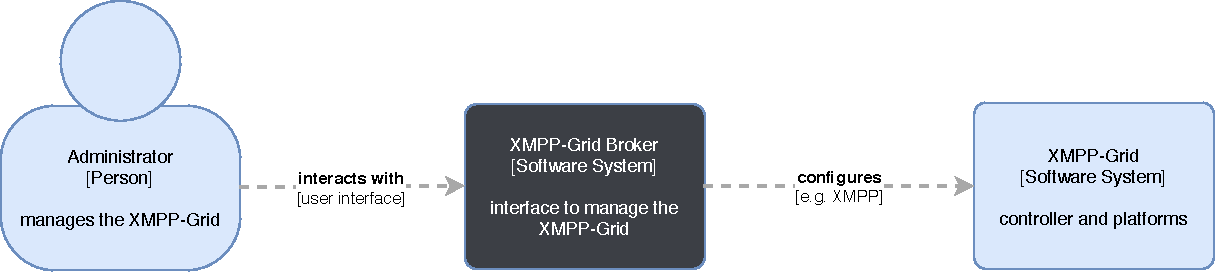
\includegraphics[width=\linewidth]{resources/architecture_context}
\caption[Architecture Context Diagram]{Architecture diagram showing the context of the XMPP grid broker application.}
\label{fig:architecturecontext}
\end{figure}


\subsection{Architectural Style and Platform}

To implement the XMPP grid broker, we evaluated three possible architecture styles:\hfill\\
An XMPP Server Plugin (e.g. extension for the Openfire XMPP server), an implementation with the Jabber Component Protocol~\cite{xep-0114} or an implementation acting as a regular XMPP client ("bot").

We decided to build an XMPP client/bot, because it is not coupled to a specific XMPP server as the Server Plugin and, in contrast to the XMPP Component, supports a strong authentication mechanism with SASL.

The full decision argument is documented in Appendix~\fullref{sec:architectural-decisions}.

\subsubsection{Platform}

The proposed XMPP client might be implemented in three different ways: as rich client application with a command line or graphical interface as illustrated in Figure~\ref{fig:architecturecontainerrichclient}, or in the form of a web application, illustrated in Figure~\ref{fig:architecturecontainerwebapplication} and \ref{fig:architecturecontainerwebproxy}.

\begin{figure}[h]
\centering
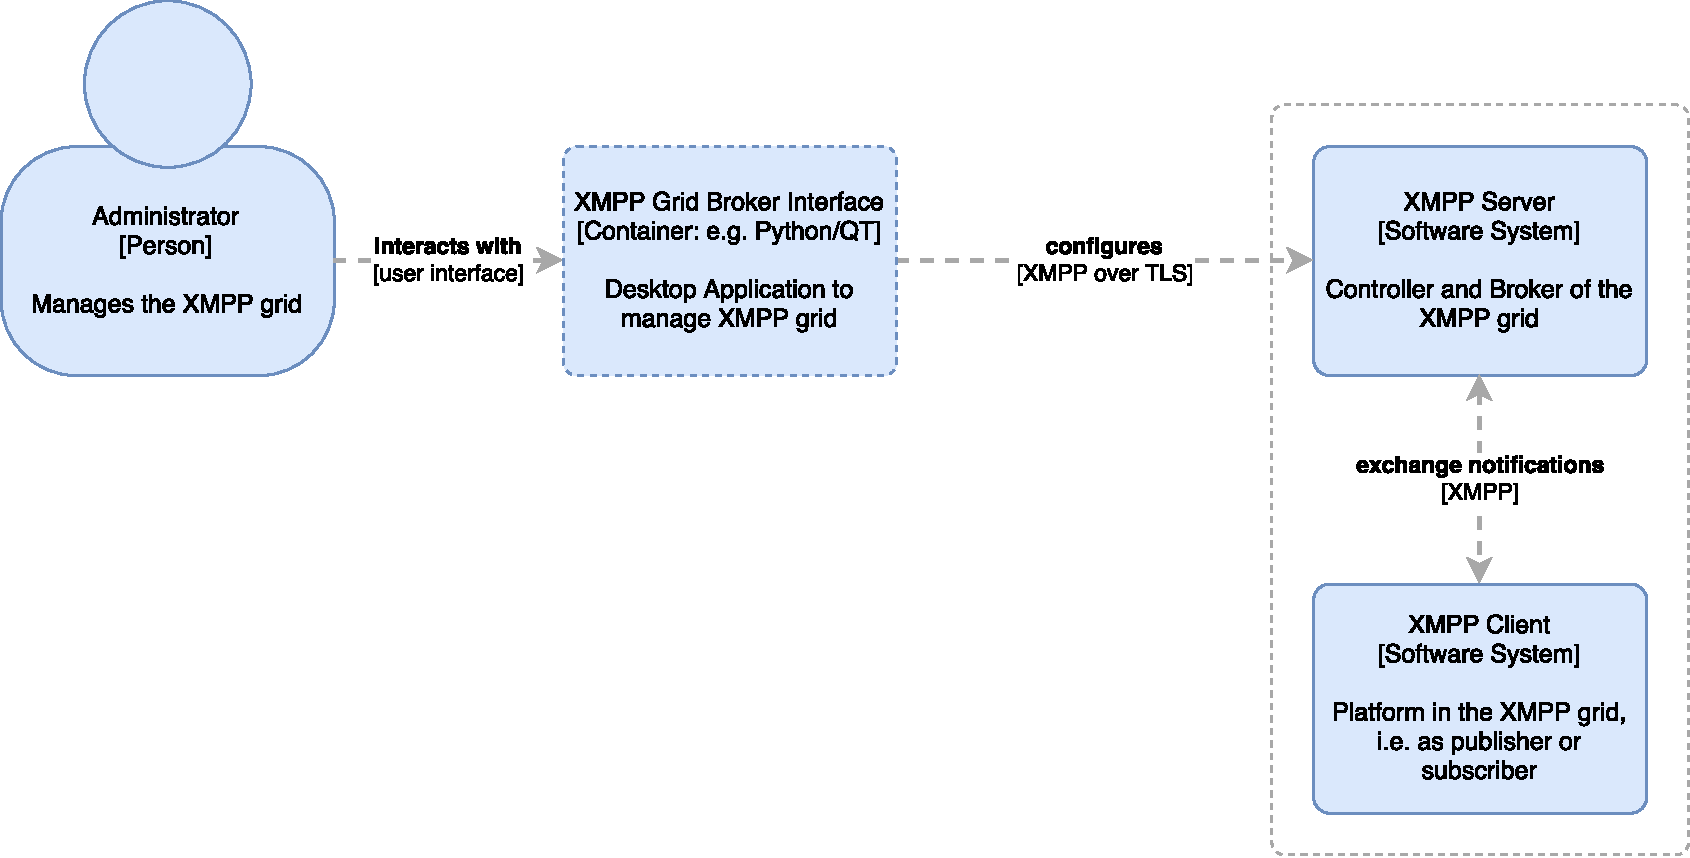
\includegraphics[width=0.7\linewidth]{resources/architecture_container_rich_client}
\caption[Architecture Container Diagram: Rich Client]{Architecture Container Diagram showing a possible rich client architecture.}
\label{fig:architecturecontainerrichclient}
\end{figure}

A web application has the significant advantage to be easily installable, upgradable and has minimal requirements on the user's side (i.e. only requires a web browser to be executed).
Therefore, we decided to implement the XMPP grid broker as web application.

\subsection{Web Application Topology}

To manage the Controller from our interface, we considered the implementation of either directly connecting to the XMPP server over WebSockets~\cite{rfc7395} or HTTP (BOSH~\cite{xep-0124}), or to communicate indirectly with the XMPP server via custom WebAPI Proxy.
These topologies are illustrated in Figure~\ref{fig:architecturecontainerwebapplication} and Figure~\ref{fig:architecturecontainerwebproxy}.

As elaborated in the according design decision (see Appendix~\ref{sec:architectural-decisions}), we decided for the direct connection via WebSockets.
This topology simplifies the implementation and deployment of the application in comparison to a WebAPI Proxy.
Additionally, WebSockets offer stateful TCP-sockets to exchange data with the XMPP server in contrast to BOSH, which uses HTTP long polling to emulate a bidirectional stream~\cite{xep-0124}.

Using the XMPP Service Discovery~\cite{xep-0030}, the XMPP server may be queried for supported features, so that only supported functionality is presented to the application user.

\begin{figure}[h]
\centering
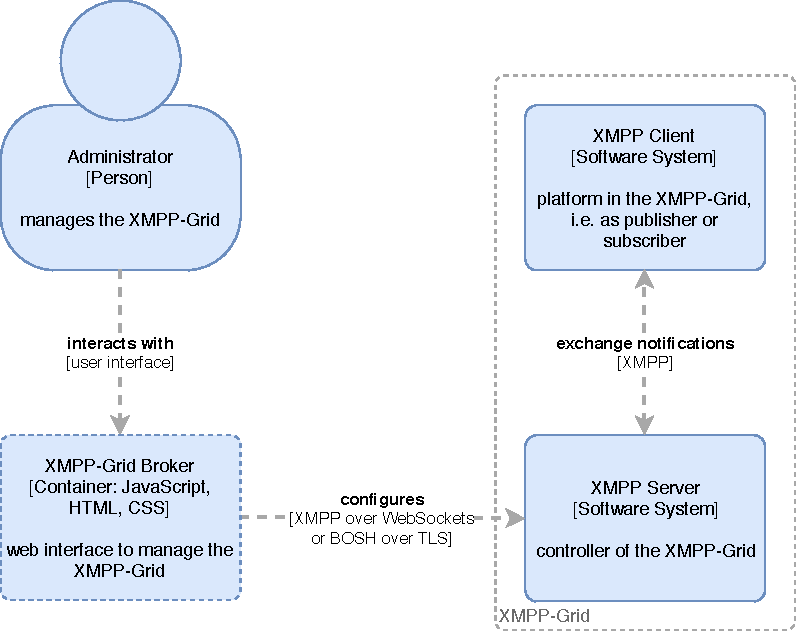
\includegraphics[width=0.7\linewidth]{resources/architecture_container_webapplication}
\caption[Architecture Container Diagram: Web Application]{Architecture Container Diagram showing the web application topology with WebSockets or BOSH.}
\label{fig:architecturecontainerwebapplication}
\end{figure}

\begin{figure}[h]
\centering
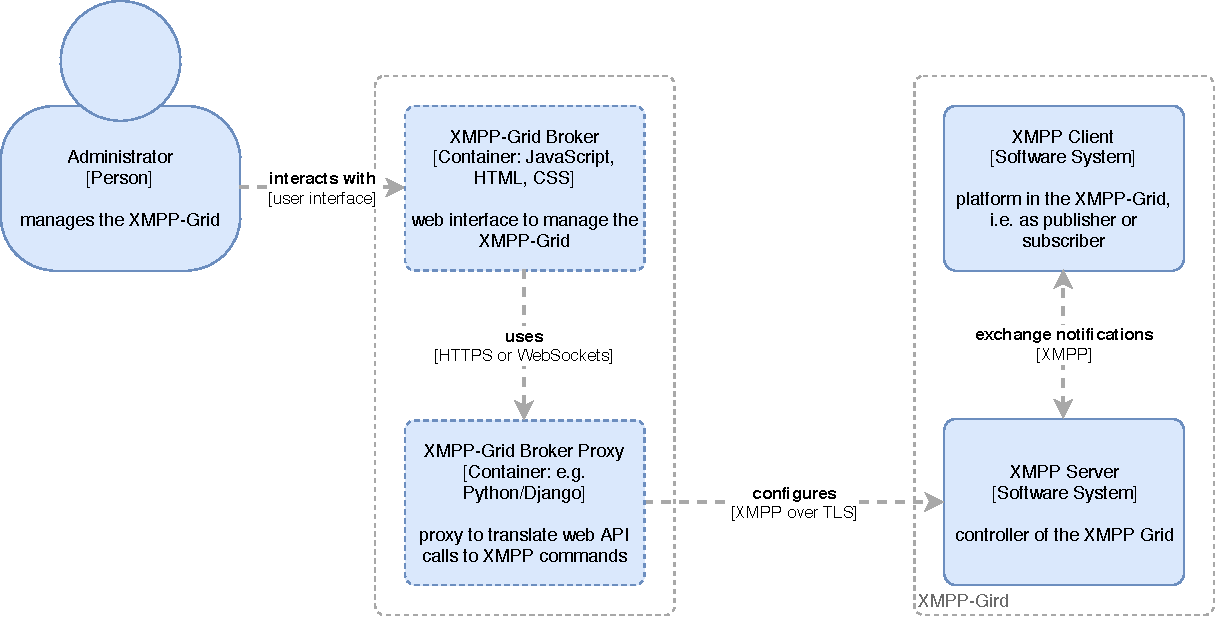
\includegraphics[width=0.7\linewidth]{resources/architecture_container_proxy.pdf}
\caption[Architecture Container Diagram: Web Proxy]{Architecture Container Diagram showing the WebAPI Proxy topology.}
\label{fig:architecturecontainerwebproxy}
\end{figure}


\subsection{Authentication and Connection Security}

XMPP uses SASL as authentication mechanism~\cite{rfc6120}.
To authenticate against the XMPP Grid Controller, we decided to use the SASL EXTERNAL~\cite{rfc4422} mechanism whenever possible to authenticate the client.

We decided against the alternative SASL authentication method, SASL SCRAM~\cite{rfc7677}, that is also recommended by in the XMPP grid draft~\cite{ietf-mile-xmpp-grid-05}.
As described in the corresponding architectural decision (Appendix~\ref{sec:architectural-decisions}), the main reason for SASL EXTERNAL is its higher level of security and and its relatively simple scaling capabilities.

SASL EXTERNAL implies that the authentication takes place on a lower layer than the actual XMPP protocol. In our case, this implies authentication over TLS, i.e.~X.509 end-user certificates as specified in RFC6120~\cite{rfc6120}.


\section{Wireframes}

We created wireframes for most screens to visualise the initial set of user stories.
They helped us to find missing requirements, most notably the support of collections.
All wireframes are listed in Appendix~\fullref{sec:wireframes}.
